\documentclass[twoside,11pt]{article}

% Any additional packages needed should be included after jmlr2e.
% Note that jmlr2e.sty includes epsfig, amssymb, natbib and graphicx,
% and defines many common macros, such as 'proof' and 'example'.
%
% It also sets the bibliographystyle to plainnat; for more information on
% natbib citation styles, see the natbib documentation, a copy of which
% is archived at http://www.jmlr.org/format/natbib.pdf

\usepackage{jmlr2e}
\usepackage{amsmath}
\usepackage{subcaption}
\DeclareMathOperator*{\argmax}{arg\,max}
\DeclareMathOperator*{\argmin}{arg\,min}

% Definitions of handy macros can go here

\newcommand{\dataset}{{\cal D}}
\newcommand{\fracpartial}[2]{\frac{\partial #1}{\partial  #2}}

% Heading arguments are {volume}{year}{pages}{submitted}{published}{author-full-names}
% \jmlrheading{1}{2020}{}{6/20}{}{Pushkar Kolhe}

% Short headings should be running head and authors last names

\ShortHeadings{ICML 2020 Workshop on Real World Experiment Design and Active Learning}{Workshop on Real World Experiment Design and Active Learning}
\firstpageno{1}

\begin{document}

\title{Batch Acquisition for Deep Bayesian Active Learning with Imperfect Oracles}

\author{\name Pushkar Kolhe \email pushkar@gatech.edu \\
       \addr Department of Interactive Computing\\
       Georgia Institute of Technology\\
       Atlanta, GA 30332, USA}

\editor{}

\maketitle

\begin{abstract}%   <- trailing '%' for backward compatibility of .sty file
Active Learning is used to maintain accuracy while reducing the training set size in many machine learning applications. However active learning approaches are not yet common in practice because they make a strong assumption on the quality of labeled data from an oracle. For machine learning applications whose goal is to estimate a model with very high confidence, we propose a framework for querying data in active learning that works with noisy oracles. In this framework we extend BatchBALD \citep{kirsch2019batchbald} to create a batch query with a control example and multiple informative examples for the task of deep Bayesian active learning. This allows us to infer the proficiency of the labeler and associate a confidence estimate while using their labels.
\end{abstract} d

\begin{keywords}
  Active Learning, Applied Machine Learning, Human-Computer Interaction
\end{keywords}

\section{Introduction}

Active Learning is a family of machine learning methods which may query the data instances to be labeled for training by an oracle (e.g., a human annotator). These methods can achieve comparable performance to passive learning methods with fewer labeled examples. Active Learning is a promising approach to improve many machine learning applications, but is is rarely used in practice due to practical challenges. One of the strong assumptions of earlier active learning methods is that the oracle is perfect, however that is often not true. Even  if  labels  come  from  human  experts, they may not always be reliable:  (i) some instances are implicitly difficult for both people and machines, and (ii) people can become distracted or fatigued over time, which introduces variability in the quality of their annotations. With the recent introduction of services like Mechanical Turk this problem has become even more relevant.

There are still many open research opportunities along these lines. In particular, how might the effect of payment influence annotation quality (i.e., if you pay a non-expert twice as much, are they sufficiently motivated to be more accurate)?  What if some instances are inherently ambiguous regardless of which annotator is used, so repeated labeling is not likely to improve matters?  In most crowd-sourcing environments,  the users are not necessarily available  “on  demand,”  thus  accurate  estimates  of  annotator  quality  may  be  difficult  to achieve  in  the  first  place,  and  might  possibly  never  be  applicable  again  since  the  model has no real choice over which to use.  In this paper we do not optimize active learning with respect to cost. We show how our labeling scheme can be used with imperfect oracles for active learning problems.

\section{Related Work}

One way to think about the problem of non-experts is agnostic active learning \cite{balcan2009agnostic}, a framework which relaxes the assumption that the oracle's labels are trustworthy, yet still has positive theoretical results. Other  recent  work  assumes  that  a  learner  may  repeat  queries  to  be  labeled  by  multiple annotators \cite{sheng2008get}. They analyze the different strategies that could be used for re-labeling. This introduces another interesting research issues.  When should the learner decide to query for the (potentially noisy) label of a new unlabeled instance, versus querying for repeated labels to de-noise an existing but suspicious training instance?  How can the learner even decide that the quality of a label is suspect?

In the context of neural networks, \cite{gupta2019learning} show how a denoising layer can be added to make active learning robust to label noises. Another approach more recently has been in designing an end-to-end framework such as \cite{platanios2020learning} where a new loss function is introduced that includes instances difficulties and predictor competencies. The authors claim that due to their framework annotators are assigned to instances they are more likely to label correctly  while performing crowdsourcing. Both these approaches introduces bias in the learning process, either by introducing a change in the model or adding new parameters in the loss function. To their credit they provide various examples and their results shows promise. In our approach we separate the process of learning from the labeling process, which means that in our approach the learning process is not biased by the actual labeling. In a practical setting someone could choose to label multiple batches together before performing one active learning loop to update the model. In our view separating the active learning and labeling process makes our approach more practical.

\cite{ipeirotis2014repeated} goes through the basics of repeated labeling and show that it is indeed useful. In their paper they discuss basic repeated labeling strategies such as majority voting, fixed round robin strategy with and without costs and selective repeated labeling. They also show that incorrectly labeled examples tend to have higher model uncertainty scores, compared to correctly labeled examples. They also introduce soft labeling and weighted labeling in the context of active learning. They conclude in their paper that selective repeated-labeling is preferable after taking into account both labeling uncertainty and model uncertainity. This conclusion has heavily influenced our approach.

% \vspace{1em}
% The main contributions of this work are:
% \begin{enumerate}
%   \item A model for modeling the proficiency of a labeler.
%   \item A method that utilizes the labelers proficiency to update beliefs on the data label.
%   \item Extending the BatchBALD algorithm to use imperfect labelers
% \end{enumerate}

\section{Background}

In this paper we focus on Bayesian Neural Networks and the MNIST example used by \cite{kirsch2019batchbald}. Compared to regular neural networks, bayesian neural networks maintain a distribution over their weights instead of point estimates. Since exact inference in bayesian neural networks is intractable, we use a variational approximation such as MC dropout \citep{gal2016dropout}. In Bayesian Neural Networks model uncertainty can be measured by an acquisition function like the Batch-BALD acquisition function and label uncertainty can be measured as the entropy of the labels for the data in our unlabelled pool. In our experiments we repeatedly go through active learning loops, that is we reinitialize the model on the available labelled data and the new data acquired after the labeling procedure. We also keep the dropout masks in MC dropout consistent while sampling from the model.

Our approach is most similar to the Completely Automated Public Turing test to tell Computers and Humans Apart (reCAPTCHA) system \cite{recaptcha}. It is a challenge response system used online to determine whether a user is a human or a computer. In it, users are asked to transcribe images into words. The reCAPTCHA system specifically challenges the user with two images. In its most simplest instantiation the system knows the trascribtion of an image, but does not know the trascribtion of the other image. When the user answers the challenge, the system verifies if the user was indeed an human from the known trascribtion and then uses the other answer as the trascribtion of the other image. In further sections we show how this labeling idea can be applied to the framework of active learning in Bayesian Neural Networks.

\subsection{Problem Setting}

We borrow and modify the problem setup from \cite{kirsch2019batchbald}. The Bayesian active learning setup consists of an unlabelled dataset $D_{pool}$, the current training set $D_{train}$, a Bayesian model $M$ with model parameters $\omega \sim p(\omega | D_{train})$, and output predictions $p(y|x, \omega, D_{train})$ for data point $x$ and prediction $y \in \{1, ..., c\}$ in the classification case. The model has been trained on $D_{train}$ and the oracle labels a data point in the unlabelled pool $x \in D_{pool}$. The goal is to obtain a certain level of prediction accuracy with the least amount of oracle queries.

At each acquisition step, a batch of data points $\{x^*_1, ..., x^*_b\}$ is selected using the BatchBALD acquisition function which scores the candidate batch of unlabelled data points $\{x^*_1, ..., x^*_b\} \in D_{pool} $ using the current model parameters $p(\omega|D_{train})$:

\begin{equation}
    \{x^*_1, ..., x^*_b\} = \argmax_{\{x^*_1, ..., x^*_b\} \in D_{pool}} \sum^b_{i=1} I(y_i; \omega | x_i, D_{train})
    \label{eq:acquisition_function}
\end{equation}

Here $I$ is the joint entropy between the data points and the model parameters as given in \cite{kirsch2019batchbald}. The acquisition function \eqref{eq:acquisition_function} requires us to test each data point using MC dropout to get the posterior for each data point. When the oracle labels on of these points it can be added to the training set. This strategy makes sense when the oracle is always correct. In this paper we relax this assumption, so we need a new strategy to gather labels.
 
We first select a candidate batch according to \eqref{eq:acquisition_function}. Then we run multiple repeated labeling events with different labelers. In each of this event we select some control queries and other candidate queries from the BatchBALD batch. The labelers proficiency is evaluated by comparing their labels with the control queries' labels. This proficiency score is then used while updating the posterior probabilities of the candidate queries. See Figure \ref{fig:query} for an example.

\begin{figure}[ht]
  \subfloat[An example candidate query for labeling. Control data points are on the top.]{
	\begin{minipage}[c][1\width]{
	   0.3\textwidth}
	   \centering
	   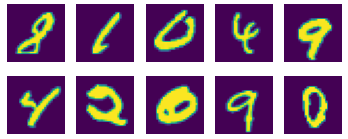
\includegraphics[width=1.0\textwidth]{figs/ex1}
	   \label{fig:query}
	\end{minipage}}
 \hfill 	
  \subfloat[Entropy decreases as a the number labels per data point increases]{
	\begin{minipage}[c][1\width]{
	   0.3\textwidth}
	   \centering
	   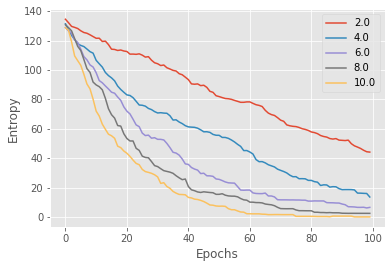
\includegraphics[width=1.0\textwidth]{figs/entropy}
	   \label{fig:entropy}
	\end{minipage}}
 \hfill	
  \subfloat[Loss converges quickly when more labels are used per data point]{
	\begin{minipage}[c][1\width]{
	   0.3\textwidth}
	   \centering
	   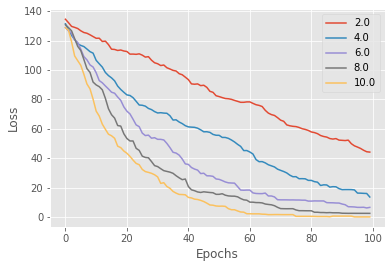
\includegraphics[width=1.0\textwidth]{figs/loss}
	   \label{fig:loss}
	\end{minipage}}
\caption{}
\end{figure}

\subsection{Modeling proficiency of the oracle}

The proficiency of the oracle is modeled as a classification loss. In this case we use the log loss between the oracle's labels and the predictions of the model.

\begin{equation}
    p = \frac{1}{N} \sum^c_{i=1} D_{KL} (y_i || \hat{y}_c)
\end{equation}

\subsection{Updating from labelers feedback}

The oracle is imperfect. So for updating the posterior probabilities of the labels of a candidate point we can use the Bayes Rule. It allows us to add a prior to the labels and the confidence in the labelers labels. Using the Bayes rule

\begin{equation*}
    P(C|D) = \frac{P(D|C)P(C)}{ \sum_{C \in \boldsymbol{C}} P(D|C)P(C)}
\end{equation*}

where $\boldsymbol{C}$ is the set of all the labels of $C$ and $D$ is the proficiency of the labeler. When multiple labelers have labeled a candidate data point, its posterior is updated using this method.

\subsection{Extending BatchBALD algorithm}

After running a few labeling loops we take the candidate data points whose entropy is below a certain acceptable threshold. In our experiments we took the candidate points below the median entropy and fed them into the training set. After that we run the active learning loops, that is we reinitialize the model using the original training set and the new data acquired after the labeling procedure. We then rerun the MC dropout to get a new candidate batch using the BatchBALD acquisition function given be \eqref{eq:acquisition_function}.

% \begin{algorithm}[tb]
%   \caption{Extend BatchBALD}
%   \label{alg:extended_batchbald}
% \begin{algorithmic}
%   \STATE {\bfseries Input:} epochs $n$, unlabelled dataset $D_{pool}$, model parameters $p(w|D_{train})$
%   \STATE $A_0 = 0$
%   \FOR{$n=1$ {\bfseries to} $n$}
%   \STATE $\boldsymbol{x_n} = BatchBALD(D_{pool}) $
%   \IF{$x_i > x_{i+1}$}
%   \STATE Swap $x_i$ and $x_{i+1}$
%   \STATE $noChange = false$
%   \ENDIF
%   \ENDFOR
%   \REPEAT
%   \STATE Initialize $noChange = true$.
%   \FOR{$i=1$ {\bfseries to} $m-1$}
%   \IF{$x_i > x_{i+1}$}
%   \STATE Swap $x_i$ and $x_{i+1}$
%   \STATE $noChange = false$
%   \ENDIF
%   \ENDFOR
%   \UNTIL{$noChange$ is $true$}
% \end{algorithmic}
% \end{algorithm}

% \begin{algorithm}[tb]
%   \caption{Bubble Sort}
%   \label{alg:example}
% \begin{algorithmic}
%   \STATE {\bfseries Input:} data $x_i$, size $m$
%   \REPEAT
%   \STATE Initialize $noChange = true$.
%   \FOR{$i=1$ {\bfseries to} $m-1$}
%   \IF{$x_i > x_{i+1}$}
%   \STATE Swap $x_i$ and $x_{i+1}$
%   \STATE $noChange = false$
%   \ENDIF
%   \ENDFOR
%   \UNTIL{$noChange$ is $true$}
% \end{algorithmic}
% \end{algorithm}

\section{Experiments}

From the analysis shown in \cite{recaptcha}, 67.87\% of the words required only two human responses to be considered correct, 17.86\% required three, 7.10\% required four, 3.11\% required five, and only 4.06\% required six or more transcribtions. Just like reCaptcha we were interested for finding out how repeated labels affect accuracy of the candidate data points. We chose to measure accuracy using entropy in the labels and log loss. We measured entropy because we are using the proficiency of the labeler to update the posterior of the labels, so a working experiment should show entropy decreasing as we get similar labels. If we get different labels for the same data point it might mean that the particular data point is ambiguous for our labelers.

After each labeling event we calculate the entropy on the labels for all candidate data points. Figure \ref{fig:entropy} shows how the entropies of the candidate batch goes down as we query more labelers. As the size of the queries increase the entropy decreases faster. Similar trends are seen in Figure \ref{fig:loss} which shows the log loss on the candidate batch.

\section{Conclusion}

We show how the BatchBALD algorithm proposed in \cite{kirsch2019batchbald} can be extended to use human in the loop for labeling, especially when the human is not an oracle and can make mistakes. We propose a new querying technique where the labelers are shown control queries along with candidate queries from the BatchBALD algorithm. Their proficiency is determine from their labels on the control queries and it is used to update the posteriors of the candidate query data points. Using this approach allows us to use labeled data points with confidence before adding them to the training set and rerunning the MC dropout pipeline to get a new candidate batch that is best for retraining the learner. 

% \newpage

% \appendix
% \section*{Appendix A.}
% \label{app:theorem}

% % Note: in this sample, the section number is hard-coded in. Following
% % proper LaTeX conventions, it should properly be coded as a reference:

% %In this appendix we prove the following theorem from
% %Section~\ref{sec:textree-generalization}:

% In this appendix we prove the following theorem from
% Section~6.2:

% \noindent
% {\bf Theorem} {\it Let $u,v,w$ be discrete variables such that $v, w$ do
% not co-occur with $u$ (i.e., $u\neq0\;\Rightarrow \;v=w=0$ in a given
% dataset $\dataset$). Let $N_{v0},N_{w0}$ be the number of data points for
% which $v=0, w=0$ respectively, and let $I_{uv},I_{uw}$ be the
% respective empirical mutual information values based on the sample
% $\dataset$. Then
% \[
% 	N_{v0} \;>\; N_{w0}\;\;\Rightarrow\;\;I_{uv} \;\leq\;I_{uw}
% \]
% with equality only if $u$ is identically 0.} \hfill\BlackBox

% \noindent
% {\bf Proof}. We use the notation:
% \[
% P_v(i) \;=\;\frac{N_v^i}{N},\;\;\;i \neq 0;\;\;\;
% P_{v0}\;\equiv\;P_v(0)\; = \;1 - \sum_{i\neq 0}P_v(i).
% \]
% These values represent the (empirical) probabilities of $v$
% taking value $i\neq 0$ and 0 respectively.  Entropies will be denoted
% by $H$. We aim to show that $\fracpartial{I_{uv}}{P_{v0}} < 0$....\\

% {\noindent \em Remainder omitted in this sample. See http://www.jmlr.org/papers/ for full paper.}


\vskip 0.2in
\bibliography{sample}

\end{document}